\section{Arkadiusz Wzorek}
\label{sec:awzorek}

\subsection{Leonhard Euler}

\textbf{Leonhard Euler} – szwajcarski matematyk i fizyk; był pionierem w wielu obszarach obu tych nauk. Jest uważany za czołowego matematyka XVIII wieku i jednego z najwybitniejszych w całej historii. Euler wniósł wkład do niemal wszystkich ówczesnych dziedzin matematyki:

\begin{itemize}
    \item[--] geometrii,
    \item[--] rachunku różniczkowego i całkowego,
    \item[--] trygonometrii,
    \item[--] algebry,
    \item[--] teorii liczb.
\end{itemize}

\noindent Poniżej (rysunek \ref{fig:euler}) portret uczonego:

\begin{figure}[htbp]
    \centering
    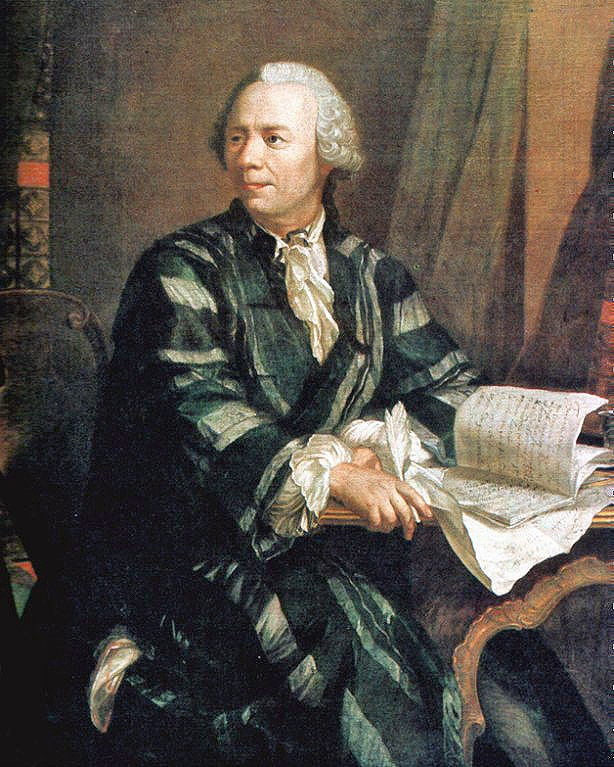
\includegraphics[width=0.5\textwidth]{pictures/euler.jpg}
    \caption{Leonhard Euler.}
    \label{fig:euler}
\end{figure}

\subsection{Wzór Eulera}

\textbf{Wzór Eulera} – wzór analizy zespolonej wiążący funkcje trygonometryczne z zespoloną funkcją wykładniczą, określany nazwiskiem Leonharda Eulera.

Niech $ x\in\mathbb{R} $, zaś $ i $ jest jednostką urojoną, wtedy wzór Eulera ma postać:
$$ e^{ix} = \cos x + i\sin x $$

\subsection{„Najpiękniejszy wzór”}
W szczególności, podstawiając $ x = \pi $, otrzymuje się równość:
$$ e^{\pi i} + 1 = 0 $$
nazywaną \textbf{tożsamością Eulera}.

Tożsamość Eulera nazywana jest często \textit{najpiękniejszym wzorem matematycznym}. Wykorzystane są w niej trzy działania arytmetyczne: dodawanie, mnożenie i potęgowanie. Tożsamość łączy pięć fundamentalnych stałych matematycznych:

\begin{enumerate}
    \item liczbę 0,
    \item liczbę 1,
    \item liczbę $ \pi $,
    \item liczbę $ e $,
    \item liczbę $ i $, jednostkę urojoną liczb zespolonych.
\end{enumerate}

Dodatkowo każde z powyższych działań oraz każda ze stałych użyte są \textit{dokładnie raz}, co więcej: wzór ten jest przedstawiony w zwyczajowej formie równania, którego prawa strona jest zerem.

\subsection{Inne szczególne przypadki}

Tabela \ref{tab:special_cases} przedstawia pozostałe ciekawe przypadki wzoru Eulera.

\begin{table}[htbp]
    \centering
    \begin{tabular}{|c|c|}
        \hline
        $ x $ & $ e^{ix} $ \\
        \hline
        $ 0 + 2k \pi$ & $ 1 $ \\
        \hline
        $ \frac{\pi}{2} + 2k \pi $ & $ i $ \\
        \hline
        $ \pi + 2k \pi $ & $ -1 $ \\
        \hline
        $ \frac{3\pi}{2} + 2k \pi $ & $ -i $ \\
        \hline
    \end{tabular}
    \caption{Inne szczególne przypadki wzoru Eulera.}
    \label{tab:special_cases}
\end{table}